\section{率失真编码定理}
\label{sec:rd-coding-theorem}

现在有两个函数：$R_{\mathrm{op}}(D)$由所有块编码决定，$R(D)$由单个符号上的优化决定。本节证明它们相等。证明分两半：任何码的码率都不能低于$R(D)$，这是下界；存在一列码以任意接近$R(D)$的码率达到失真$D$，这是可达性。

本节的设定是：$\mathcal{X}$与$\hat{\mathcal{X}}$有限，信源无记忆，失真按式~\eqref{eq:rd-block-distortion}可分，并且$d_{\max}=\max_{x,\hat{x}}d(x,\hat{x})<\infty$（有限字母表上这自动成立）。由于每个符号的失真都不低于它的最佳重构，任何码都满足$\mathbb{E}d_n\geq D_{\min}$，所以$D<D_{\min}$时没有可达对，只需讨论$D\geq D_{\min}$。

\begin{theorem}[率失真编码定理]
\label{thm:rd-coding}
在上述设定下，对每个$D\geq D_{\min}$，
\begin{equation}
  R_{\mathrm{op}}(D)=R(D).
  \label{eq:rd-coding-theorem}
\end{equation}
\end{theorem}

定理只说极限。它不告诉我们给定块长$n$时最好的码有多好，也不给出能在合理时间内运行的编码器；这两点在本节末尾再谈。

\subsection{码率的下界}
\label{sec:rd-converse}

任取一个$(n,M)$码，记编号为$J=f_n(X^{n})$，重构为$\hat{X}^{n}=g_n(J)$，期望失真为$\Delta=\mathbb{E}d_n(X^{n},\hat{X}^{n})$。目标是证明
\begin{equation}
  \frac{\log_2M}{n}\geq R(\Delta).
  \label{eq:rd-converse}
\end{equation}
思路是图~\ref{fig:rd-converse-chain}：所有源符号都挤过一个只有$M$个值的编号；把每一对$(X_i,\hat{X}_i)$单独拿出来，得到$n$个单符号测试信道；它们的平均又是一个测试信道，失真恰好是$\Delta$。

\begin{BookInlineFigure}
  \centering
  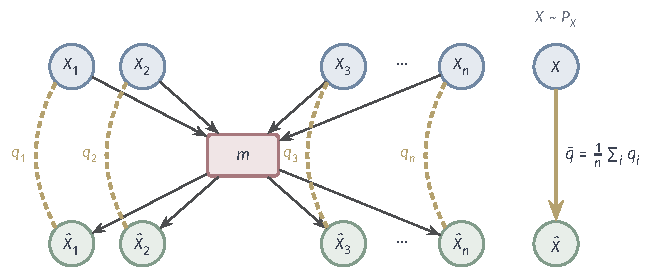
\includegraphics[width=110mm]{figures/07-probability/05-source-coding/tikz/rd-converse-chain/figure.pdf}
  \caption{下界证明的结构。蓝色源符号全部经过红框中的编号$J$（至多$M_n$个值）才到达绿色重构。黄色虚线表示每一对$(X_i,\hat{X}_i)$的条件分布，它是一个单符号测试信道$q_i$；右侧是它们的平均$\bar{q}$，输入仍服从$P_X$。}
  \label{fig:rd-converse-chain}
\end{BookInlineFigure}

\paragraph{第一步：编号限制信息}
$X^{n}\to J\to\hat{X}^{n}$构成Markov链：$\hat{X}^{n}$是$J$的函数，给定$J$后不再依赖$X^{n}$。由第~\ref{chap:information-measures}章的数据处理不等式，后处理不增加信息，
\[
  I(X^{n};\hat{X}^{n})\leq I(X^{n};J)\leq H(J)\leq\log_2M .
\]
第二个不等号是$I(X^{n};J)=H(J)-H(J\mid X^{n})$与条件熵非负，第三个是$J$只取$M$个值。

\paragraph{第二步：拆成单个符号}
把互信息写成源块的熵减去给定重构后的条件熵。信源无记忆，各$X_i$独立，联合熵可加：
\[
  H(X^{n})=\sum_{i=1}^{n}H(X_i).
\]
条件熵用链式法则逐个展开，再用“条件越多熵越小”去掉多余的条件：
\[
  H(X^{n}\mid\hat{X}^{n})=\sum_{i=1}^{n}H(X_i\mid X_1,\dots,X_{i-1},\hat{X}^{n})\leq\sum_{i=1}^{n}H(X_i\mid\hat{X}_i).
\]
两式相减，得到
\[
  I(X^{n};\hat{X}^{n})\geq\sum_{i=1}^{n}\bigl(H(X_i)-H(X_i\mid\hat{X}_i)\bigr)=\sum_{i=1}^{n}I(X_i;\hat{X}_i).
\]

\paragraph{第三步：平均成一个测试信道}
记第$i$个位置的条件分布为
\[
  q_i(\hat{x}\mid x)=\mathbb{P}(\hat{X}_i=\hat{x}\mid X_i=x),
\]
对$p(x)>0$的$x$定义，其余$x$任取一个分布。因为每个$X_i$都服从$P_X$，第$i$对的互信息就是$I(P_X,q_i)$。第$i$个位置的平均失真记为$\Delta_i$，它就是$q_i$在式~\eqref{eq:rd-test-distortion}中的失真。

令$\bar{q}=\frac1n\sum_iq_i$，由引理~\ref{lem:rd-mi-convex}（推广到$n$个信道的凸组合，按$n$归纳），
\[
  \frac1n\sum_{i=1}^{n}I(P_X,q_i)\geq I(P_X,\bar{q}).
\]
失真对测试信道线性，$\bar{q}$的平均失真是$\frac1n\sum_i\Delta_i$。由式~\eqref{eq:rd-block-distortion}，它正是$\Delta$。所以$\bar{q}$在$R(\Delta)$的可行集合中，$I(P_X,\bar{q})\geq R(\Delta)$。

把三步连起来：
\[
  \log_2M\geq I(X^{n};\hat{X}^{n})\geq\sum_{i=1}^{n}I(P_X,q_i)\geq n\,I(P_X,\bar{q})\geq n\,R(\Delta),
\]
这就是式~\eqref{eq:rd-converse}。

\paragraph{从单个码到渐近下界}
设$(R',D)$可达，相应码列的期望失真为$\Delta_n$，$\limsup_n\Delta_n\leq D$。对任意$\varepsilon>0$，$n$充分大时$\Delta_n\leq D+\varepsilon$，由式~\eqref{eq:rd-converse}与$R$非增，
\[
  \frac{\log_2M_n}{n}\geq R(\Delta_n)\geq R(D+\varepsilon).
\]
取上极限得$R'\geq R(D+\varepsilon)$。由定理~\ref{thm:rd-existence}，$R$在$[D_{\min},\infty)$上连续，令$\varepsilon\to0$得$R'\geq R(D)$。所以$R_{\mathrm{op}}(D)\geq R(D)$。

\paragraph{两个假设各用在哪里}
无记忆性用在第二步与第三步：$H(X^{n})=\sum_iH(X_i)$需要独立，$I(X_i;\hat{X}_i)=I(P_X,q_i)$需要每个$X_i$的分布都是$P_X$。可分失真用在第三步的最后：$\bar{q}$的失真等于块失真，靠的是块失真等于逐符号失真的平均。

去掉无记忆性，单符号的$R(D)$就不再是正确答案。设$Y\sim\operatorname{Bern}(0.3)$，令$X_1=X_2=\dots=X_n=Y$。每个$X_i$的分布仍是$\operatorname{Bern}(0.3)$，单符号的$R(0)$仍是$h_2(0.3)\approx0.881$。可是整块只有两种可能，用$1$\,bit传送$Y$就能零失真重构，码率$1/n\to0$。第二步中
\[
  H(X^{n})=h_2(0.3),\qquad \sum_{i=1}^{n}H(X_i)=n\,h_2(0.3),
\]
前者远小于后者，链条在这里断开。带记忆的信源需要按块定义信息量再取极限，本章不讨论。

\subsection{可达的码率}
\label{sec:rd-achievability}

下界说码率不能低于$R(D)$。反方向要构造码。直接设计最优码本很难，下面的办法是随机撒点：按最优测试信道的重构边缘独立地生成很多码字，证明平均而言总有一个码字离源块足够近，再由平均推出确定的好码本存在。

\paragraph{为什么随机码本能覆盖}
取达到$R(D)$的测试信道$q$（定理~\ref{thm:rd-existence}保证存在），它的重构边缘为$r=r_q$，$I=I(P_X,q)=R(D)$。对一个典型的源块$x^{n}$，随机抽一个码字$Y^{n}$，各分量独立服从$r$，它“恰好与$x^{n}$配成像是由$q$产生的一对”的概率有多大？

对一对$(x,\hat{x})$，记\term{信息密度}（information density）
\begin{equation}
  \imath(x,\hat{x})=\log_2\frac{q(\hat{x}\mid x)}{r(\hat{x})},\qquad
  \imath_n(x^{n},\hat{x}^{n})=\sum_{i=1}^{n}\imath(x_i,\hat{x}_i),
  \label{eq:rd-information-density}
\end{equation}
只在$q(\hat{x}\mid x)>0$处定义。按联合分布$p(x)q(\hat{x}\mid x)$取期望，由式~\eqref{eq:rd-test-information}，$\mathbb{E}\,\imath(X,\hat{X})=I$。$\imath_n$越大，块对$(x^{n},\hat{x}^{n})$在$q$下比在“$\hat{x}^{n}$与$x^{n}$无关”时越可能出现，倍数是$2^{\imath_n}$。

若$(X_i,\hat{X}_i)$独立地按$p(x)q(\hat{x}\mid x)$产生，大数律使$\frac1n\imath_n$集中在$I$附近，图~\ref{fig:rd-info-density}展示了这种集中。于是“像是由$q$产生的”块对，其$\imath_n$约为$nI$，从$r^{n}$中独立抽到这样的$\hat{x}^{n}$的概率约为$2^{-nI}$。要有把握至少抽中一个，码字数应超过$2^{nI}$，也就是码率略高于$I=R(D)$。

\begin{BookInlineFigure}
  \centering
  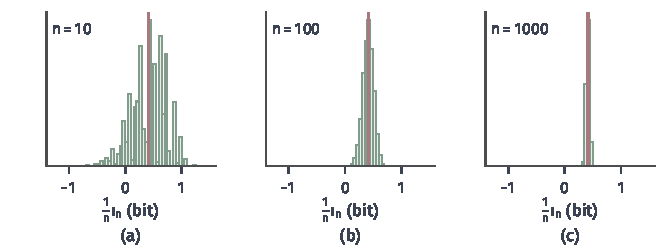
\includegraphics[width=112mm]{figures/07-probability/05-source-coding/matplotlib/rd-info-density/figure.pdf}
  \caption{$\operatorname{Bern}(0.3)$信源、Hamming失真、$D=0.1$的最优联合分布下，每符号信息密度$\frac1n\imath_n$的直方图（绿），块长$n=10,100,1000$，各$20000$个块，随机种子$722$。单个符号的$\imath$只取$0.363$、$-2.807$、$-1.585$、$1.585$四个值；红线是均值$I=R(0.1)\approx0.412$。$n=1000$时样本标准差约为$0.029$。}
  \label{fig:rd-info-density}
\end{BookInlineFigure}

下面把这个估计写成不等式。对$\gamma>0$与$D'\geq0$，令
\[
  \mathcal{A}=\Bigl\{(x^{n},\hat{x}^{n}):\ q^{n}(\hat{x}^{n}\mid x^{n})>0,\ \imath_n(x^{n},\hat{x}^{n})\leq\log_2\gamma,\ d_n(x^{n},\hat{x}^{n})\leq D'\Bigr\},
\]
其中$q^{n}$是$q$逐符号作用于整块的条件概率，即各分量$q(\hat{x}_i\mid x_i)$的乘积。$\mathcal{A}$中的块对失真达标，信息密度又不过大，称为\term{失真典型集}（distortion-typical set）。对固定的$x^{n}$，把与它配成$\mathcal{A}$中块对的重构块全体记为$\mathcal{A}(x^{n})$。

\begin{lemma}[随机码本的覆盖]
\label{lem:rd-covering}
设码字$C_1,\dots,C_M$相互独立，各分量独立服从$r$，并与$X^{n}$独立。令$(X^{n},\hat{X}^{n})$按$\prod_ip(x_i)q(\hat{x}_i\mid x_i)$分布。则
\begin{equation}
  \mathbb{P}\bigl(\text{没有}C_m\in\mathcal{A}(X^{n})\bigr)\leq\mathbb{P}\bigl((X^{n},\hat{X}^{n})\notin\mathcal{A}\bigr)+\mathrm{e}^{-M/\gamma}.
  \label{eq:rd-covering}
\end{equation}
\end{lemma}

\begin{proof}
固定$x^{n}$，令
\[
  g(x^{n})=\sum_{\hat{x}^{n}\in\mathcal{A}(x^{n})}q^{n}(\hat{x}^{n}\mid x^{n}),
\]
它是按测试信道重构时落入$\mathcal{A}(x^{n})$的概率。对$\hat{x}^{n}\in\mathcal{A}(x^{n})$，由式~\eqref{eq:rd-information-density}，
\[
  r^{n}(\hat{x}^{n})=q^{n}(\hat{x}^{n}\mid x^{n})\,2^{-\imath_n(x^{n},\hat{x}^{n})}\geq\frac{1}{\gamma}\,q^{n}(\hat{x}^{n}\mid x^{n}),
\]
其中$r^{n}(\hat{x}^{n})=\prod_ir(\hat{x}_i)$。对$\mathcal{A}(x^{n})$求和，单个码字落入$\mathcal{A}(x^{n})$的概率至少是$g(x^{n})/\gamma$。

$M$个码字独立，全部落空的概率是
\[
  \Bigl(1-\mathbb{P}\bigl(C_1\in\mathcal{A}(x^{n})\bigr)\Bigr)^{M}\leq\Bigl(1-\frac{g(x^{n})}{\gamma}\Bigr)^{M}\leq\exp\Bigl(-\frac{M\,g(x^{n})}{\gamma}\Bigr),
\]
最后一步用了$1-u\leq\mathrm{e}^{-u}$。

再把指数关于$g$放大成线性函数。对$c\geq0$，$t\mapsto\mathrm{e}^{-ct}$在$[0,1]$上凸，图像在两端点连线之下：
\[
  \mathrm{e}^{-ct}\leq(1-t)+t\,\mathrm{e}^{-c}\leq1-t+\mathrm{e}^{-c},\qquad t\in[0,1].
\]
取$c=M/\gamma$，$t=g(x^{n})$，全部落空的概率至多为$1-g(x^{n})+\mathrm{e}^{-M/\gamma}$。

最后对$x^{n}$按$P_X^{n}$平均。$1-g(X^{n})$的期望正是$(X^{n},\hat{X}^{n})\notin\mathcal{A}$的概率，于是得到式~\eqref{eq:rd-covering}。
\end{proof}

式~\eqref{eq:rd-covering}右端两项各有分工。第一项是测试信道本身“不典型”的概率，由大数律控制；第二项是码字太少、撒网不够密的代价，只要$M$远大于$\gamma\approx2^{nI}$就可忽略。

\begin{theorem}[可达性]
\label{thm:rd-achievability}
在本节设定下，对$D\geq D_{\min}$与任意$R'>R(D)$，$(R',D)$可达。于是$R_{\mathrm{op}}(D)\leq R(D)$。
\end{theorem}

\begin{proof}
取$\delta>0$，令$I=R(D)$，$q$为达到$R(D)$的测试信道，$\mathbb{E}_qd\leq D$。下面分四步。

\emph{码本大小。}令$\gamma_n=2^{n(I+\delta)}$，$M_n=\lceil2^{n(I+2\delta)}\rceil$，$D'=D+\delta$。码率满足
\[
  \frac{\log_2M_n}{n}\leq\frac{\log_2\bigl(2^{n(I+2\delta)}+1\bigr)}{n}\to I+2\delta .
\]

\emph{覆盖失败的概率。}$(X_i,\hat{X}_i)$独立同分布，$\imath(X_i,\hat{X}_i)$只取有限个值，均值为$I$；$d(X_i,\hat{X}_i)$有界，均值不超过$D$。由第~\ref{chap:laws-of-large-numbers}章的弱大数律，
\[
  \mathbb{P}\Bigl(\frac1n\imath_n>I+\delta\Bigr)\to0,\qquad \mathbb{P}\bigl(d_n>D+\delta\bigr)\to0 .
\]
所以式~\eqref{eq:rd-covering}的第一项趋于零。第二项中$M_n/\gamma_n\geq2^{n\delta}$，故
\[
  \mathrm{e}^{-M_n/\gamma_n}\leq\exp(-2^{n\delta})\to0 .
\]记右端为$\varepsilon_n$，$\varepsilon_n\to0$。

\emph{随机码的平均失真。}用最近码字编码器。只要有一个$C_m\in\mathcal{A}(X^{n})$，最近码字的失真就不超过$D+\delta$；否则失真不超过$d_{\max}$。对源与码本一起取期望，
\[
  \mathbb{E}\bigl[d_n(X^{n},\hat{X}^{n})\bigr]\leq D+\delta+d_{\max}\,\varepsilon_n .
\]

\emph{从随机码本到确定码本。}左端是对随机码本取平均后的期望失真，平均值不超过某个数，至少有一个码本的期望失真不超过这个数。于是对每个充分大的$n$，存在确定的$(n,M_n)$码，期望失真不超过$D+\delta+d_{\max}\varepsilon_n$。对较小的$n$随便取一个码，不影响上极限。这说明$(I+2\delta,D+\delta)$可达。

$\delta$可以任意小。给定$R'>I$，对一切满足$I+2\delta\leq R'$的$\delta$，$(R',D+\delta)$都可达。下面的对角线论证说明$(R',D)$也可达。
\end{proof}

\paragraph{边界点的极限处理}
设对每个$k$，$(R',D+\tfrac1k)$可达，相应的码列为$\mathcal{C}^{(k)}$。由上极限的定义，存在$N_k$，使$n\geq N_k$时$\mathcal{C}^{(k)}$中块长为$n$的码满足
\[
  \frac{\log_2M_n}{n}\leq R'+\frac1k,\qquad \mathbb{E}d_n\leq D+\frac2k .
\]
可以取$N_1<N_2<\cdots$。对$N_k\leq n<N_{k+1}$，块长$n$时使用$\mathcal{C}^{(k)}$中的码。$n\to\infty$时所用的$k$也趋于无穷，所以新码列满足式~\eqref{eq:rd-achievable}，$(R',D)$可达。可达区域在这个意义下是闭的。

至此$R_{\mathrm{op}}(D)\leq R(D)$，与第~\ref{sec:rd-converse}节的下界合起来，定理~\ref{thm:rd-coding}得证。在$D=D_{\min}$处，下界用到了$R$在端点的右连续，可达性则靠这里的极限处理；两边都不要求在端点处有特别的构造。

\paragraph{有限块长与计算代价}
定理只保证极限。先给极限一个记号：由定理~\ref{thm:rd-zero-rate}，$R$在$[D_{\min},D_{\max}]$上严格递减，它的反函数记为$D(R)$，称为\term{失真率函数}（distortion-rate function），表示码率为$R$时能达到的最小失真。雨天记录中$D(0.5)\approx0.0742$，即$R(D)=0.5$的解。

图~\ref{fig:rd-finite-codes}(a)用穷举给出$n\leq4$时每种码本大小下最好的码，它们都在曲线上方不远处，码率$\tfrac12$时最好的失真从$n=2$的$0.15$降到$n=4$的约$0.136$，离$D(0.5)$仍有距离。图~\ref{fig:rd-finite-codes}(b)是按证明构造的随机码本：码率固定为$\tfrac12$，块长到$36$时平均失真约为$0.097$，仍明显高于极限。

\begin{BookInlineFigure}
  \centering
  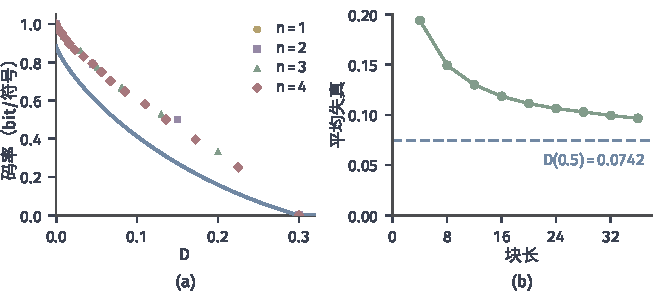
\includegraphics[width=112mm]{figures/07-probability/05-source-coding/matplotlib/rd-finite-codes/figure.pdf}
  \caption{$\operatorname{Bern}(0.3)$信源与Hamming失真下的有限块长码。(a)对$n=1,2,3,4$穷举全部码本，每种码本大小$M$下期望失真最小的码（不同颜色与形状），横坐标为失真，纵坐标为$\log_2M/n$；蓝线是$R(D)$。(b)码率$\tfrac12$的随机码本，码字各分量独立服从$\operatorname{Bern}(0.265)$（码率$\tfrac12$对应的最优重构边缘），最近码字编码；每个$n$用$40$个码本、每个码本$250$个源块估计平均失真，随机种子$722$。蓝色虚线是$D(0.5)\approx0.0742$。}
  \label{fig:rd-finite-codes}
\end{BookInlineFigure}

收敛慢的原因可以从证明中看出：$\frac1n\imath_n$与$d_n$的波动按$n^{-1/2}$缩小，要让它们都落在$\delta$以内，$n$要远大于$\delta^{-2}$。计算上，最近码字编码要在$2^{nR}$个码字中搜索，$n=36$、$R=\tfrac12$时已有约$2.6\times10^{5}$个码字。证明给出的是存在性，构造搜索代价低的好码是另一个问题，本章不讨论。
